\usetikzlibrary{calc}
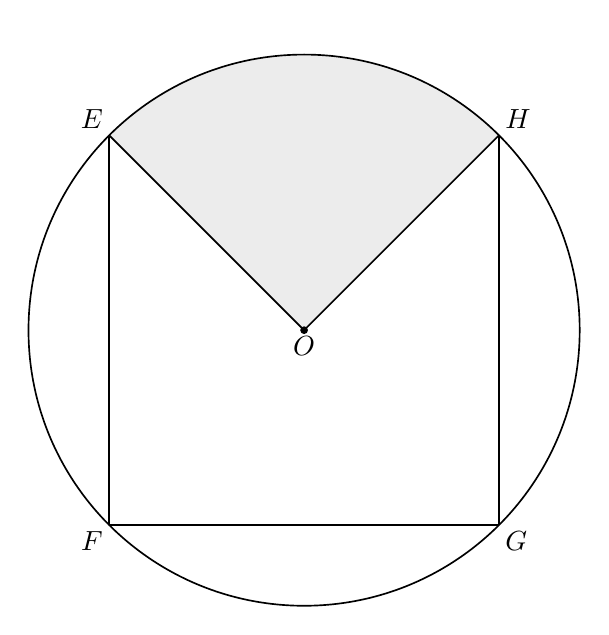
\begin{tikzpicture}[x=1cm,y=1cm,line width=.6pt,font=\normalsize]
\coordinate (O) at (0,0);
\coordinate (E) at (-2.47487,2.47487);
\coordinate (H) at (2.47487,2.47487);
\coordinate (F) at (-2.47487,-2.47487);
\coordinate (G) at (2.47487,-2.47487);
\fill[gray!15] (O)--(E) arc[start angle=135,end angle=45,radius=3.5cm]--cycle;
\draw (O) circle[radius=3.5cm];
\draw (E)--(F);
\draw (F)--(G);
\draw (G)--(H);
\draw (O)--(E);
\draw (O)--(H);
\node[above left=2pt,inner sep=0pt] at (E) {$E$};
\node[above right=2pt,inner sep=0pt] at (H) {$H$};
\node[below left=2pt,inner sep=0pt] at (F) {$F$};
\node[below right=2pt,inner sep=0pt] at (G) {$G$};
\node[below=2pt,inner sep=0pt] at (O) {$O$};

% Explicit named circle-center points, painted after all region fills.
\fill (O) circle[radius=1.4pt];
\end{tikzpicture}
